\section{脅威モデル}
\label{sec:dns-tunneling}
本章では,はじめにDNSの概要について述べる.\\
次に,本研究における脅威モデルであるDNSトンネリングについて説明する.

\subsection{DNSの概要}
\label{sec:dns-protocol}

DNSは,インターネットにおけるドメイン名に関連づけられたリソースレコードを解決するシステムである.
インターネット上のホストの識別には,本来IPアドレスを用いるが,10進数表記のIPv4(``93.184.216.34")や16進数表記のIPv6(``2606:2800:220:1:248:1893:25c8:1946")は,人が認識するには容易ではない.
このような時,DNSを用いてドメイン名にIPアドレスが関連づけていた場合,DNSがIPアドレスとの変換処理を行ってくれるため,ユーザはドメイン名のみ認知していれば済む.
このように名前解決の機能を担うDNSは,インターネットの利活用において極めて重要であり,現在のインターネットを支える根幹技術の一つである.

DNSは,クライアント・サーバアーキテクチャで構成され,機能に応じて3つのサービスに分類することができる.
\begin{itemize}
 \item スタブリゾルバ
 \vspace{-3mm}
 \item フルサービスリゾルバ
 \vspace{-3mm}
 \item 権威サーバ
\end{itemize}

スタブリゾルバは,名前解決の問い合わせるを依頼するクライアントノードである.
フルサービスリゾルバ(キャッシュサーバ・リカーシブサーバとも呼称される)は,スタブリゾルバからの名前解決問い合わせに対して,次に説明する権威サーバに実際に問い合わせるクライアントノードである.
また,過去に問い合わせた情報をキャッシュする機能があり,これによって何度も問い合わせられる情報を権威サーバに問い合わせずに即座にスタブリゾルバに応答することができる.
フルサービスリゾルバ自身は,``root.hints"というルート権威サーバとそのアドレスが対応づけられたファイルに基づいて,ルート権威サーバのアドレスを解決する.
権威サーバは,リソースレコードを保持するサーバノードであり,フルサービスリゾルバからの問い合わせ依頼に応答する.

DNSは,
権威サーバは,単一ではなく,ドメインの階層構造に基づいて
DNSは,階層ごとに名前空間を分割させた識別子の分散管理システムである.
このシステムは,ルートを頂点として,その下層に独自の名前空間を保持するドメインをツリー状に連結されていく構造をとる.
各ドメインは,権威サーバによってドメインの名前空間が管理される.
ドメインの名前空間はゾーンと呼ばれ,そのドメインに位置づく権威サーバによって管理される.
DNSには委譲の仕組みがあり,権威サーバは自身が管理するゾーンについてドメインが枝分かれしていっている場合,下層の権威サーバにゾーンを管理を譲ることができる.
一般にルートの直下で構成されるドメインをTLD(Top Level Domain)と言い,``com."や``net."などがある.
さらにその下層には,SLD(Second Level Domain)が続き,TLDからn番目(n $\mid$ n $\in$ $\mathbb{N}$)のラベルが第nレベルドメインと序列していく具合である.
TLDを大別すると,``.com"や``.net"をはじめとした特定分野別のgTLD(global Top Level Domain),``.jp"や``.ch"のような国ごとに割り当てられているccTLD(Co\\untry Code Top Level Domain)の二つに分けられる.

ドメイン名は,ドット区切りでラベルを連結形式で表記され,一般にルートを意味する最も右のドットは省略される.
ドメイン名は,ルートと区切り文字を除いて最大が253bitである.
ラベルは,各ドメインを表し,数字とアルファベットおよびハイフン(``-")の文字列から表記される最大長63bitで定義される.

\begin{figure}[h]
 \centering
 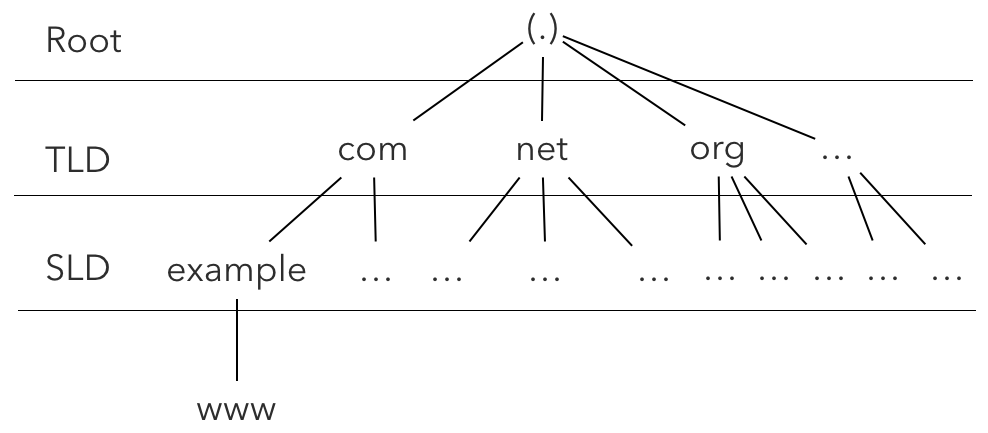
\includegraphics[width=12.0cm]{figure/dns-architecture.png}
 \caption{ドメインの名前空間}
 \label{fig:dns-architecture}
\end{figure}

ルートを頂点とするドメインの階層構造に基づいて,ドメインごとに管理するゾーンを委譲することで分散したデータベース

DNSでは,ルートを頂点とする階層構造で構成されるドメインに基づいて,ドメインごとに管理するゾーンを委譲することで分散してデータベースを保持
複数のサーバによる協調に基づいて機能を実現しており,リソースレコードと呼ばれるドメイン名に関連づけられた情報は複数のサーバに分散して管理されている.
これには,
は,複数のサーバが管理するドメインのゾーンを委譲という仕組みによって分割していく


その解決策として登場したのが,管理するドメインをゾーンで切り出し権限を委譲していく分散的な階層構造を持つDNSである.


クライアントから``www.example.com"のIPv4アドレスについて問い合わせられた場合を考える.
はじめに,クライアントであるスタブリゾルバは,スタブリゾルバと同一セグメント内のフルサービスリゾルバもしくは,ネットワークセグメントに依らずインターネット上のどのクライアントからもアクセスできるパブリックなフルサービスリゾルバ(オープンリゾルバ,パブリックリゾルバとも呼称される)に問い合わせる.
フルサービスリゾルバははじめに,ドメイン名が``www.example.com"で,リソースレコードが``A"の応答レコードがキャッシュにあるかどうかを判別する.
キャッシュにヒットした場合にはキャッシュの情報をクライアントに応答され,ヒットしなかった場合には,root.hintsファイルを参照しルート権威サーバにリクエストパケットを転送する.
クエリ(問い合わせ)を受け取ったルート権威サーバは,ルートゾーン内の``com"ドメインが委譲された権威サーバのアドレスを応答する.
次に,フルサービスリゾルバは,``com"ドメインが委譲された権威サーバに対し同様のクエリを転送する.
``com"ドメインを管理する権威サーバは,同様にして,``com"ゾーン内の``example.com"が委譲された権威サーバのアドレスを応答する.
フルリゾルバは,``example.com"ドメインを委譲された権威サーバ宛に同様のクエリを転送する.
``example.com"ゾーンを管理する権威サーバは,保持するゾーンファイルからクエリされたドメインのリソースレコードについて探索し,探索の結果としてレコード情報をフルサービスリゾルバに応答する.
フルサービスリゾルバは,権威サーバからの応答されたレコード情報のTTL(Time To Live)の期間レコード情報をキャッシュしたのち,クライアントのスタブリゾルバに結果を応答する.
このようにして,再帰的な問い合わせの仕組みに基づき名前解決がとり行われる.

\begin{figure}[h]
 \centering
 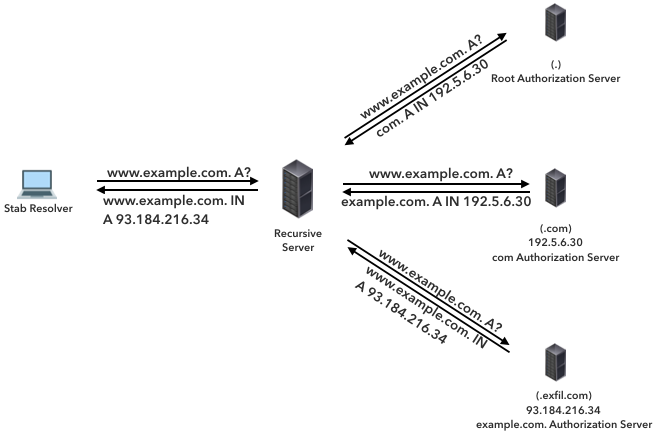
\includegraphics[width=12.0cm]{figure/dns-name-resolution.png}
 \caption{DNSによる名前解決}
 \label{fig:dns-name-resolution}
\end{figure}

%TLDごとに登録するプロセスや必要書類,金額は異なり,上位


ドメイン名に関連づけられる情報は,リソースレコード(Resorce Record, RR)と呼ばれる.
リソースレコードは,タイプが定義されており,目的ごとに使用されるタイプが異なる.
最も一般的なレコード,Aレコードタイプは,ドメインに対してIPv4アドレスを関連づけるために使用される.
名前解決において,クライアントはドメイン名とそのドメインに関連づけられたリソースレコードを指定する.
これによって,クライアントは,ドメインに関連づけられたリソースレコード情報を取得することができる.
表~\ref{tab:resource-record}は,主要なリソースレコードである.
\begin{table}[htb]
 \centering
  \begin{tabular}{ccc}
    \toprule
		\textbf{タイプ} & \textbf{値} & \textbf{意味} \\
    \midrule
    A & 1 &  ホストのIPv4アドレス \\
    NS & 2 & 権威サーバ \\
    MF & 4 & メール転送サーバ \\
    CNAME & 5 & 別名 \\
    SOA & 6 & 権威ゾーンの開始 \\
    NULL & 10 & NULL(実験用) \\
    PTR & 12 & ドメイン名のポインター(逆引き) \\
    HINFO & 13 & ホスト情報 \\
    MINFO & 14 & メールボックスおよびメールリスト情報 \\
    MX & 15 & メール交換 \\
    TXT & 16 & 任意文字列 \\
    \bottomrule
  \end{tabular}
 \caption{主要リソースレコード一覧}
 \label{tab:resource-record}
\end{table}


%リソースレコードのタイプごとの使用頻度を知りたい
% タイプごとの説明を充実させるのは,重要かもしれない


\subsection{DNSトンネリング}
DNSトンネリングは,DNSをデータ転送のメディアとした秘匿通信手法の総称である.
第~\ref{sec:dns-protocol}節で示す通り,DNSは,ドメイン名とそのドメイン名に関連づけられたリソースレコードのレコード情報を解決するシステムであり,現代のインターネットにおいて極めて重要な役割を担うネットワークプロトコルである.
% DNSのトラフィック量
このため,DNSはトラフィックがフィルタリング・モニタリングされにくいプロトコルの一つでもある.
しかし,DNSのデザインは,クライアントサーバアーキテクチャに基づき,クライアントのスタブリゾルバと権威サーバが直接やり取りされるため,の問い合わせ情報が権威サーバに転送されるため,
転送される仕組みは,データ転送の仕組みでもある.
過去のインシデントでは,権威サーバをデータ回収のサーバとして利用するケースや,次~\ref{sec:dns-infiltration}項の流入通信とを組み合わせて,命令サーバとの相互通信の流出方向の通信手段として利用されてきた.
\subsubsection{データ流出}
\label{sec:dns-exfiltration}
DNS Exfiltrationは,再帰問い合わせの仕組みによって,DNSクエリがコンテンツを保持する権威サーバに転送される仕組みをを利用した手法.
これによって,クライアントから権威サーバを宛先とする方向に対して任意のデータを転送することができる.
データを転送するためのキャリアは,DNSクエリのQuestion SectionのQNAME内のラベルである.
第~\ref{sec:dns}節で示すように,ドメイン名には一つのラベルあたり63bit,全体で253bitという制約がある.
すなわち,DNS Exfiltrationによって転送できるデータ量の最大は253bitである.
他方で,DNSの名前解決の仕組みはインターネットの利活用において必要不可欠であるため,多くの組織においてDNSのトラフィックがフィルタリングされることはほとんどない.
このような性質をもつDNSを利用することで,悪意を持つユーザがなんらかの方法で潜伏した組織内部のネットワークから情報を流出させる際の手法として,他のネットワークプロトコルに比べて都合が良い.

DNS Exfiltrationにおいて,データを転送する際の宛先ノードは特定のゾーンを管理する権威サーバである.
例えば,あるローカルネットワーク内に位置づくノードからグローバルネットワーク内の``exfil.com"という権威サーバにデータを転送することを考える.
一般に,転送するデータをQNAMEにおけるラベルに埋め込む際には,Base Encoding~\cite{rfc4648}のような変換規則によるエンコード処理が施される.
この処理によって,転送データがバイナリデータである際にも転送効率上げたり,ラベルの文字列制約を満たさないデータも転送することができる.
また,メッセージの意味抽出を困難にするためのトリックとして用いられる.
変換された文字列は,



この権威サーバは,``exfil.com"以下の全ての名前空間をゾーンとして管理することができる.
データを転送する際のキャリアとなるのは,DNSクエリの``exfil.com"以下のラベルである.
DNSのラベルは,数字・アルファベット・先頭以外でハイフン(``-")という文字列の制約があるため,任意の文字列をそのまま注入することは困難である.
任意の文字列を文字列エンコーディングの手法で変換させ,用意できた文字列をQNAMEに含め,適当なリソースレコードタイプを指定すれば,宛先となる権威サーバにデータが転送される.
最後に,ラベルを同一の文字列エンコーディングアルゴリズムでデコードすることで,元のデータを受け取ることができるという具合である.
このようにして,DNSの名前解決の仕組みを応用することで,任意の権威サーバに任意の文字列を転送することができる.
これがDNS Exfiltrationの動作メカニズムである.
図~\ref{fig:dns-exfiltration}に,DNS Exfiltrationのメカニズムを図解した様子である.

\begin{figure}[h]
 \centering
 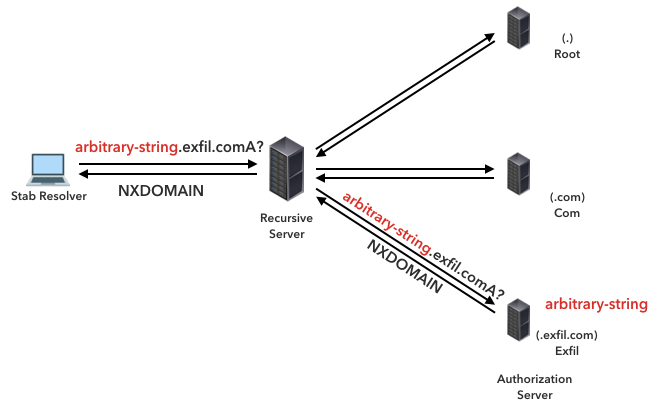
\includegraphics[width=12.0cm]{figure/dns-exfiltration.png}
 \caption{arbitrary-stringという任意の文字列が,DNSクエリのラベル部を用いて,事前に用意した権威サーバ(exfil.com)に転送される様子}
 \label{fig:dns-exfiltration}
\end{figure}

%1998年4月,DNSトンネリングの手法は,NmapのBugtraqメーリングリストにて初めて公になったとされている\cite{bugtraq}.

\subsubsection{データ流入}
\label{sec:dns-infiltration}
DNS Infiltrationは,DNS Exfiltrationと逆方向の権威サーバからクライアント方向にデータを転送する手法である.
この手法は,DNSのリソースレコードに任意の文字列が含められる設計になっていることを利用したものである.
リソースレコードのタイプは多種多様であるが,ゾーンファイルを自由に編集できる現在のDNSエコシステムでは,ドメイン名との関わりに関係なく任意の情報をドメイン名に関連づけることが可能である.
DNS Infiltrationを実施するには,送信元となる権威サーバのドメイン名に,適当なリソースレコードのタイプ(E.g. TXT)に転送したい文字列を登録しておくことで,そのドメイン名をQNAMEとしてそのレコードタイプを問い合わせることで,クライアントのもとでデータを回収することができるという具合である.
DNSのリソースレコードを転送キャリアとする流入通信のメカニズムを図解した様子が,図~\ref{fig:dns-infiltration}である.

\begin{figure}[h]
 \centering
 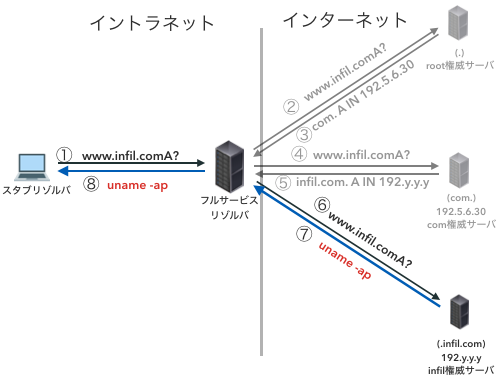
\includegraphics[width=10.0cm]{figure/dns-infiltration.png}
 \caption{TXTレコードに登録された情報について,DNSクエリで問い合わせることで権威サーバから命令情報を取得している様子}
 \label{fig:dns-infiltration}
\end{figure}

% Null タイプは,厳密に定義されておらず,実験用としか表現されていない.しかし,全体のタイプのうち,20%を示す程度に頻繁に使用されるタイプのである.

\subsection{検知に基づく既存対策手法}
本節では,DNSトンネリングに対するこれまでの対策手法について説明する.
% 検知に基づく手法の現在までの程度を淡々と示す.
\subsubsection{特徴量}
DNSトンネリングの手法を用いる場合,いくつかの特徴が現れることがある.
Bornら~\cite{born}は,DNSトンネリングにおけるクエリ内のドメイン名に出現する文字の出現頻度を着目
することで,正規のドメイン名とDNS Exfiltrationメソッドによって生成されたドメイン名とを分類のに有用であることを明らかにした(2010).
著者らは,正規のドメインであれば英語のような自然言語における文字の出現頻度と高い相関があることに加えて,エントロピーと文字列分布に高い相関があることも明らかにした.


\subsubsection{閾値推定}
\subsubsection{機械学習に基づくモデル}
%\subsubsection{パターンマッチング}
%\subsubsection{同一ドメインあたりのクエリ頻度}
%\subsubsection{Qnameにおける文字列分布}
%\subsubsection{Qnameにおける長さとエントロピー}
%\subsubsection{課題 : Low ThroughputなTunnelingに対する検知手法}
DNSトンネリングメソッドを使用した時のDNSクエリは,第~\ref{sec:dns-tunneling}項で述べるような特性が出現する.
この性質に基づき,これまでに多数の検知手法が提案されてきた.
